\documentclass{siproblemset}

\usepackage{multicol}
\usepackage{xcolor}

% SI Session Information
\course{MTH 1321}
\sessionnum{4}
\sessiondate{2/1/21}

\warmup{Concept Review}
\topic{Determining Continuity}
\topic{Introduction to Indeterminate Forms}
\cooldown{Classifying Discontinuities}

% Worksheet Information
\title{Continuity, Limits of \linebreak Continuous Functions}
\sections{Section 2.4-2.5a}
\withnamespace

\begin{document}
    \maketitle
    
    \activity{Warmup}{Concept Overview}{Try these problems \textbf{alone} as your peers join the session.}{15 minutes}
    
    \frq{Define continuity. List the three criteria for a function to be continuous at $x=a$.}
    \Tinysp
    
    \frq{List the three criteria for a function to be left- and right-continuous at $x=a$.}
    \Tinysp
    
    \frq{Name the three common types of discontinuities and sketch an example (graph) of each.}
    \Smallsp
    
    \frq{Name some of the basic functions which are continuous on their domains.}
    \Smallsp
    
    \frq{What are the indeterminate forms?}
    \tinysp
    
%    \mcq{Evaluate the following limits by using the Basic Limit Laws. $$\lim\limits_{x\to2}g(x)=3~~~\text{and}~~~\lim\limits_{x\to2}h(x)=-2$$}{
%        \task $\lim\limits_{x\to2}\dfrac{g(x)+5x}{h(x)^2}$
%        \Hugesp
%        \task $\lim\limits_{x\to2}\frac12h(x)\sqrt{g(x)}$
%        \Largesp
%    }
%    
    \pagebreak
    \activity{Activity 1}{Determining Continuity}{Work together in your \textbf{breakout rooms} to answer these questions.}{30 minutes}
    
    \begin{multipartquestion}
        Determine the intervals of continuity on the following graphs. At points of discontinuity, state if the function is left- or right-continuous at that point and the type of discontinuity.
        \frq{}
        \mbox{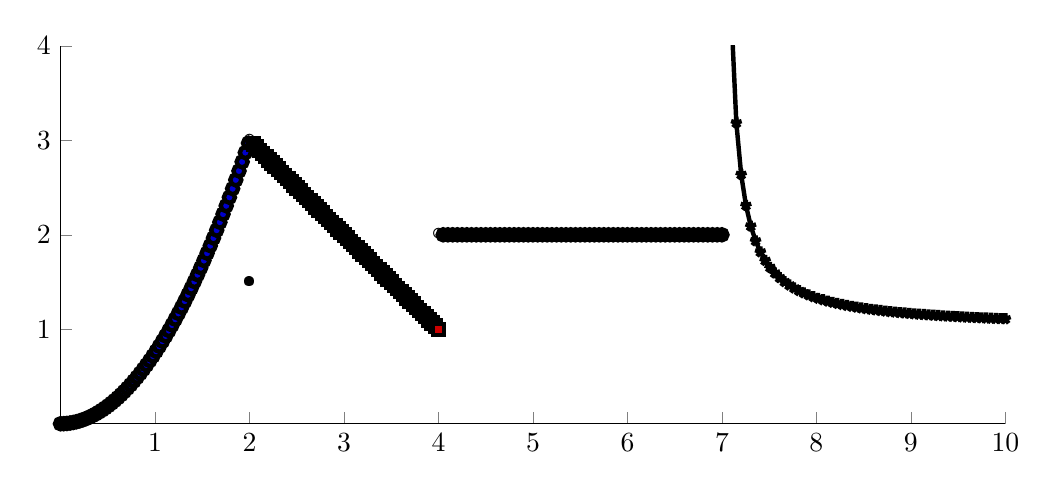
\begin{tikzpicture}[baseline=(current bounding box.north)]
            \begin{axis}[
                x=1.2cm,
                y=1.2cm,
                xmin=0,
                xmax=10,
                ymin=0,
                ymax=4,
                axis x line*=middle,
                axis y line*=middle,
                every axis plot/.append style={ultra thick},
                samples=60
                ]
                \addplot+[black, domain=0:1.99] {3/4*x^2};
                \node at (2,3) {$\circ$};
                \node at (2,1.5) {\textbullet};
                \addplot+[black, domain=2.04:4] {-x+5};
                \node at (4,1) {\textbullet};
                \node at (4,2) {$\circ$};
                \addplot+[black, domain=4.05:7] {2};
                \node at (7,2) {\textbullet};
                \addplot+[black, domain=7:10] {1/(3*(x-7))+1};
            \end{axis}
        \end{tikzpicture}}
        \tinyspace
        \frq{}
        \mbox{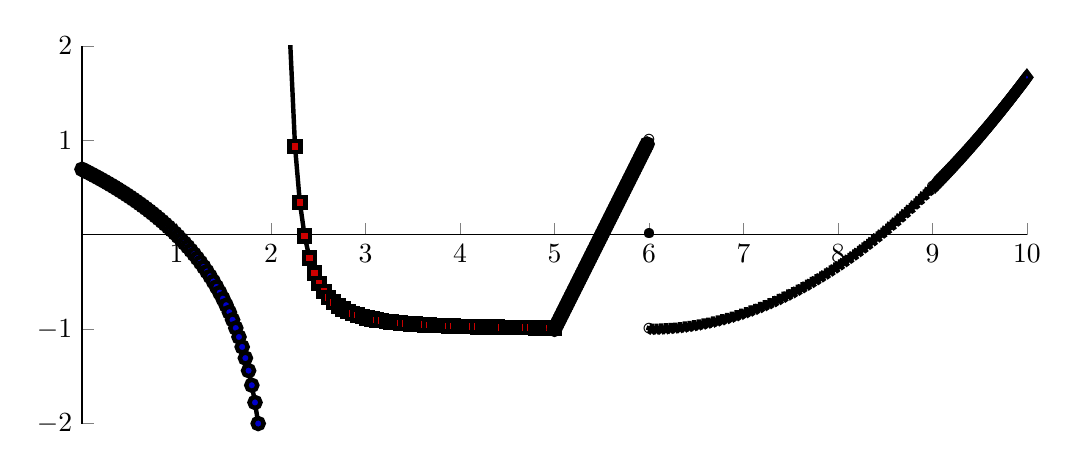
\begin{tikzpicture}[baseline=(current bounding box.north)]
            \begin{axis}[
            x=1.2cm,
            y=1.2cm,
            xmin=0,
            xmax=10,
            ymin=-2,
            ymax=2,
            axis x line*=middle,
            axis y line*=middle,
            every axis plot/.append style={ultra thick},
            samples=60
            ]
            \addplot+[black, domain=0:2] {ln(-(x-2))};
            \addplot+[black, domain=2:5,restrict y to domain =-5:5] {1/(8*(x-2)^2)-1};
            \node at (5,-1) {\textbullet};
            \addplot+[black, domain=5:5.98] {2*x-11};
            \node at (6,1) {$\circ$};
            \node at (6,0) {\textbullet};
            \node at (6,-1) {$\circ$};
            \addplot+[black, domain=6.03:8.97] {1/6*(x-6)^2-1};
            \node at (9,0.5) {$\circ$};
            \addplot+[black, domain=9.03:10] {1/6*(x-6)^2-1};
            \end{axis}
            \end{tikzpicture}}
        \tinyspace
    \end{multipartquestion}
    \pagebreak
    
    \mcq[2]{Find the points of discontinuity of the given function. State the type of discontinuity and if the function is left- or right-continuous at those point(s). If there are no points of discontinuity, state so explicitly. Justify your answers.}{
        \task $g(x)=\dfrac{x+2}{3-x}$
        \hugesp
        \task $a(b)=\dfrac{1}{b^2-9}$
        \hugesp
        \task $f(x)=\sqrt{x^2-2}$
        \hugesp
        \task $h(x)=\begin{cases}
        x^2 & x < 1\\
        4-3x &1 \leq x \leq 2\\
        \sqrt{x-2} & x < 2
        \end{cases}$ 
        
    }

\pagebreak
    

    \activity{Activity 2}{Limits and Indeterminate Forms}{Work together in your \textbf{breakout rooms} to answer these questions.}{30 minutes}

%    \frq{Determine where the given function is discontinuous. Determine the left- and right-hand limits at those points. Hint: To evaluate the one-sided limits, you will first need to rewrite the term with the absolute value using the information above and simplify the resulting expression.}
%    $$f(x) = \dfrac{(1-x)(x+2)}{\abs{x+2}}$$
%    \pagebreak

    \mcq{Evaluate the following limits. If an indeterminate form is found, state the form and use algebra to solve the limit. Explicitly state if a limit approaches $\pm \infty$. If you have extra time, determine the one-sided limits for all limits that do not exist.}{
        \task $\lim\limits_{x\to 2}\dfrac{x-3}{x^2-4x+4}$
        \Smallsp
        \task $\lim\limits_{t\to0}\dfrac{1-e^{2t}}{1-e^t}$
        \Smallsp
        \task $\lim\limits_{x\to 9}\dfrac{x-9}{\sqrt{x}-3}$
        \Smallsp
        \task $\lim\limits_{x\to 16^+}\dfrac{1}{\sqrt{x}-4}-\dfrac{8}{x-16}$
        \Smallsp
    }
    \pagebreak
    
    \activity{Cooldown}{Classifying Discontinuities}{Answer these questions as a large group.}{15 minutes}
    
    \frq{Describe the behavior of $\lim\limits_{x\to c^\pm}f(x)$ and $f(c)$ at each type of discontinuity.}
    \Smallsp
    
    \begin{multipartquestion}
        Are the following functions continuous at $x=k$? If they are not, state the type of discontinuity and whether the function is left- or right-continuous (or neither) at $x=k$.
        \frq{$h(k)=5~;~\lim\limits_{x\rightarrow k^+}h(x)=5~;~\lim\limits_{x\rightarrow k^-}h(x)=2$}
        \Smallsp
        \frq{$f(k)=4~;~\lim\limits_{x\rightarrow k}f(x)=4$}
        \Smallsp
        \frq{$g(k)=6~;~\lim\limits_{x\rightarrow k}g(x)=-2$}
        \Smallsp
        \frq{$q(k)=3~;~\lim\limits_{x\rightarrow k^+}q(x)=-6~;~\lim\limits_{x\rightarrow k^-}q(x)=-\infty$}
        \Smallsp
    \end{multipartquestion}
\end{document}